We have implemented our approach in \whoop, a prototype infrastructure that combines static lockset analysis with state-of-the-art compilation and sequential verification techniques to (i) soundly analyse Linux kernel modules for data races and (ii) accelerate a plugged-in precise bug finder. Figure~\ref{fig:whoop}

\begin{figure*}
\centering
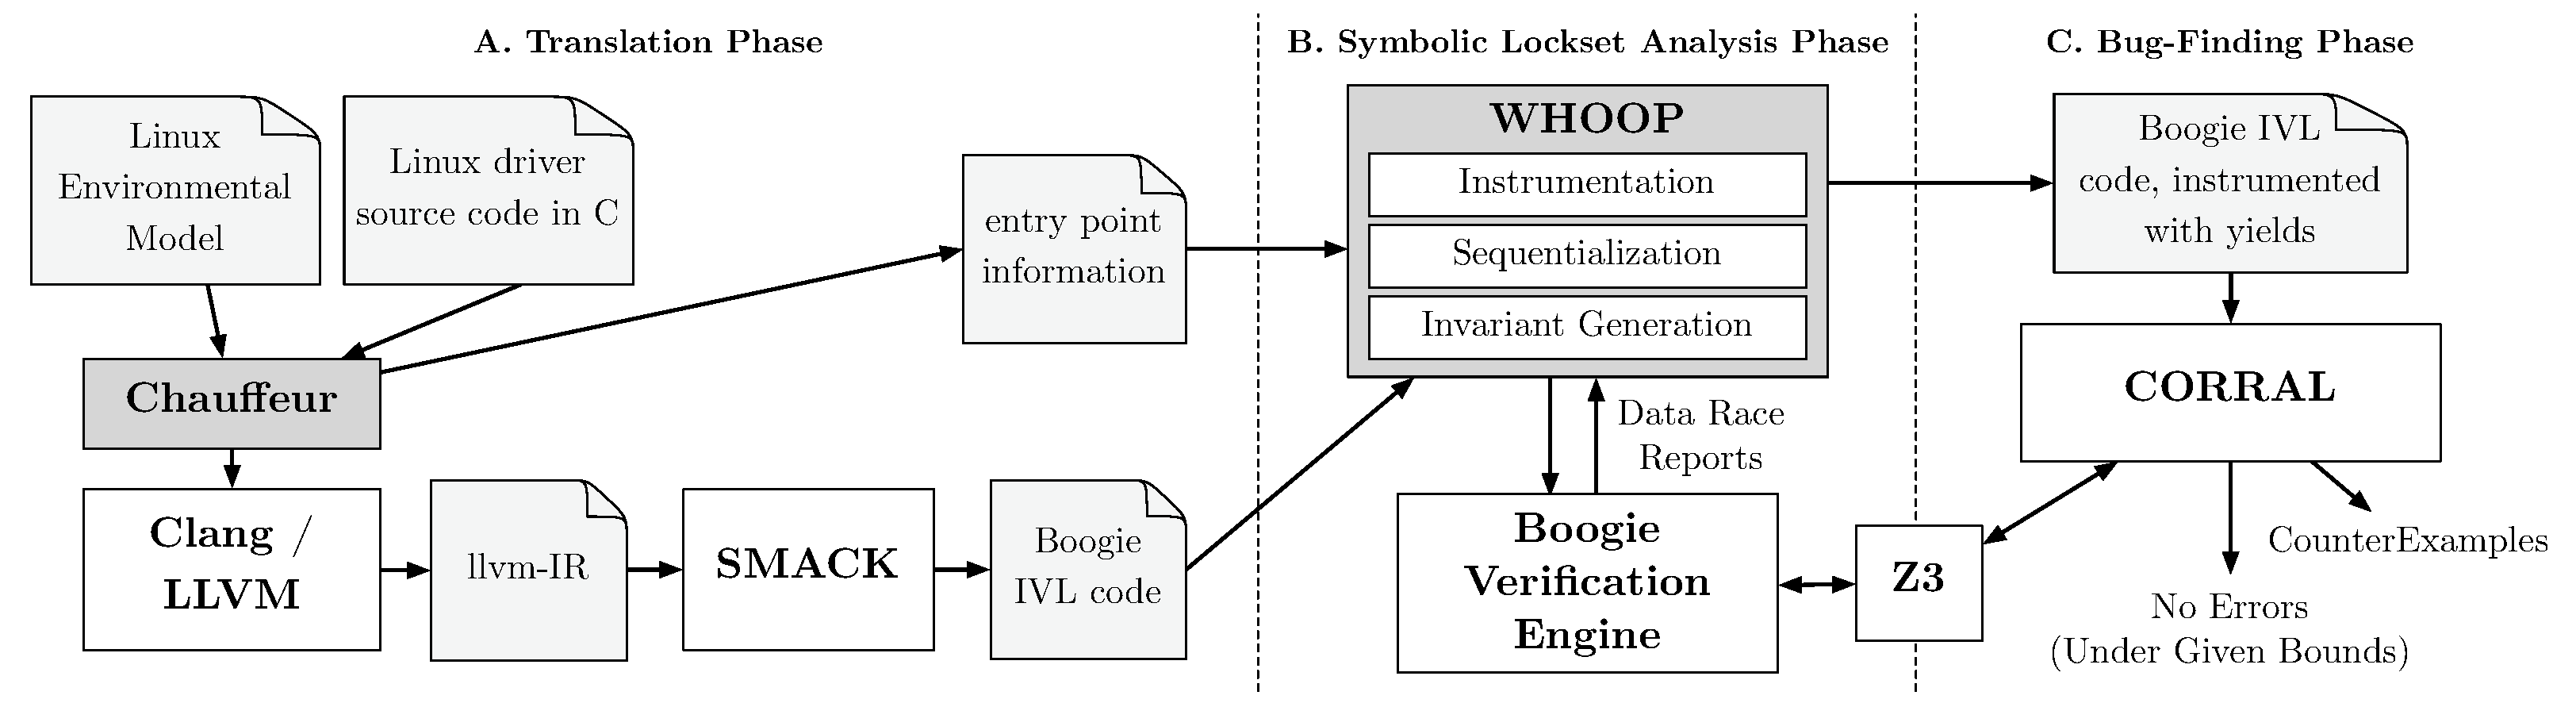
\includegraphics[width=.99\linewidth]{img/whoop.pdf}
\caption{The \textsc{Whoop} infrastructure, empowered by state-of-the-art compilation (Clang/LLVM and SMACK) and verification (Boogie and Corral) tools}
\label{fig:whoop}
\end{figure*}

The proof sketch behind our static lockset analysis is given in Section~\ref{proof}. The verification technique is described in more detail in Section~\ref{method}. The summarisation that we perform to achieve scalability is discussed in Section~\ref{summarisation}. Various optimisations that we perform to achieve precision are described in Section~\ref{optimisations}. Finally, the prototype implementation of our approach as the practical tool \textsc{Whoop} is presented in Section~\ref{implementation}.

\subsection{Static Pairwise Lockset Analysis}
\label{spla}

We now present \emph{static pairwise lockset analysis}, a novel verification technique for proving data race freedom in Linux kernel modules. The key idea behind our approach is that we can verify absence of data races by (i) deriving a sound \emph{sequential} model that \emph{over-approximates} the originally concurrent program, (ii) instrumenting it for lockset analysis and race checking, and (iii) asserting that all write/read accesses to the same shared resource are consistently protected by at least one common lock. The immediate benefit is that our approach not only avoids reasoning about thread interleavings, and thus has the potential to scale well, but also allows the reuse of existing sequential verification techniques.

\subsection{Static Lockset Analysis Proof Sketch}
\label{proof}

We now formalise our approach to verifying data race freedom in a kernel module by statically analysing its locksets. Let $\{\mathit{ep}_{1}, \mathit{ep}_{2}, \dotsc, \mathit{ep}_{n}\}$ be all the entry points of a module, and let $\{\ell_{1}, \ell_{2}, \dotsc, \ell_{k}\}$ be all the locks used by this module. Although we assume that the number of locks is finite and with a known bound, we argue that this assumption is realistic: all modules that we have studied so far in the Linux kernel have only a small number of locks (typically one). Indeed, the Linux device driver book~\cite{corbet2005linux} advocates the use of as few locks as possible to avoid introducing unnecessary complexity and synchronisation bugs that arise from careless fine-grained locking. The actual Linux kernel employs sophisticated fine-grained locking, but this is part of the environment which is abstracted away in our models.

For each entry point $\mathit{ep}_{i}$, we compute its lockset $\mathit{LS}_{i}$ that associates each memory location $m$ to the set of locks that are always held when $m$ is accessed during the execution of $\mathit{ep}_{i}$. Furthermore, for each entry point $\mathit{ep}_{i}$, we compute its read-set $R_{i}\lbrack m\rbrack \rightarrow \{true, false\}$ and its write-set $W_{i}\lbrack m\rbrack \rightarrow \{true, false\}$, which map each $m$ to true if and only if $\mathit{ep}_{i}$ reads or writes respectively to $m$ during some execution. In the actual implementation we avoid the use of quantifiers by using a different lockset, read-set and write-set for each shared memory location. \PDComment{any concrete reference that quantifiers might be harder for SMT solving?}

\begin{theorem}
\label{theorem:locksets}
For each pair of entry points $\mathit{ep}_{i}, \mathit{ep}_{j}\in \{\mathit{ep}_{1}, \mathit{ep}_{2}, ..., \mathit{ep}_{n}\}$, where $i$ may be equal to $j$, and for each memory location $m$, if $(W_{i}\lbrack m\rbrack \vee W_{j}\lbrack m\rbrack) \wedge (W_{i}\lbrack m\rbrack \vee R_{j}\lbrack m\rbrack) \wedge (R_{i}\lbrack m\rbrack \vee W_{j}\lbrack m\rbrack) \implies (\mathit{LS}_{i}\lbrack m\rbrack \cap \mathit{LS}_{j}\lbrack m\rbrack \not= \varnothing)$, then the kernel module with entry points $\{\mathit{ep}_{1}, \mathit{ep}_{2}, \dotsc, \mathit{ep}_{n}\}$ is free from data races.
\end{theorem}

A sketch of how the above theorem can be proved is as follows. Suppose there are in fact entry points $\mathit{ep}_{i}$ and $\mathit{ep}_{j}$ that can race on a memory location $m$. By our hypothesis, there exists at least one lock, say $\ell$, which belongs to both $\mathit{LS}_{i}$ and $\mathit{LS}_{j}$. By the definition of a lockset, this means that $\ell$ is held during the access to $m$ by both $ep_1$ and $ep_2$. As a result, $m$ \emph{must} be unlocked and locked between the two accesses, which contradicts that the pair of accesses is racing.

\subsection{Verification Method}
\label{method}

\begin{table*}
\small
\begin{center}
\begin{tabular}{lll}
\textbf{Statement}           & \textbf{Logger's Instrumentation}      & \textbf{Checker's Instrumentation} \\
\noalign{\smallskip}\toprule
\textbf{lock}(m);              & \textbf{add\_lock}(CL, m);                        & \textbf{add\_lock}(CL, m); \\
\noalign{\smallskip}\hline\noalign{\smallskip}
\textbf{unlock}(m);          & \textbf{remove\_lock}(CL, m);                  & \textbf{remove\_lock}(CL, m); \\
\noalign{\smallskip}\hline\noalign{\smallskip}
\multirow{2}{*}{x := *ptr;} & LS$\lbrack $ptr$\rbrack :=$ LS$\lbrack $ptr$\rbrack$ $\cap$ CL; & \textbf{assert}(W$\lbrack $ptr$\rbrack \implies$ CL $\cap$ LS$\lbrack $ptr$\rbrack \not= \varnothing$); \\
\noalign{\smallskip}
                                       & \textbf{havoc}(x);                                 & \textbf{havoc}(x); \\
\noalign{\smallskip}\hline\noalign{\smallskip}
\multirow{2}{*}{*ptr := x;} & LS$\lbrack $ptr$\rbrack :=$ LS$\lbrack $ptr$\rbrack$ $\cap$ CL; & \multirow{2}{*}{\textbf{assert}(CL $\cap$ LS$\lbrack $ptr$\rbrack \not= \varnothing$);} \\
\noalign{\smallskip}
                                       & W$\lbrack $ptr$\rbrack := true;$ &
\end{tabular}
\end{center}
\caption{Logger and Checker statements to be instrumented in each pair of entry points. The \texttt{havoc(x)} statement assigns a nondeterministic value to \texttt{x}.}
\label{tab:instrumentation}
\end{table*}

Our verification technique begins by performing \emph{two-thread reduction}, a sound abstraction that removes all but two arbitrary threads, each running an entry point of the originally concurrent program, and then performs \emph{pairwise sequentialisation}, which combines the two arbitrary threads in a single sequential pair. This is achieved by replacing the \texttt{return} statement of the first entry point with a \texttt{goto} statement that jumps execution to the first statement of the second entry point. This process repeats until all pairs of entry points have been sequentialised. To achieve soundness, each time an entry point performs a read access to a shared resource, we return a nondeterministic value. This over-approximates any effects from all the unmodeled threads on the device driver shared state.

Next, we split each pair into two distinct analysis regions: the \emph{logger}, which contains all the statements from the first entry point; and the \emph{checker}, which contains all the statements from the second entry point. The logger and the checker are then instrumented according to Table~\ref{tab:instrumentation}. The two regions directly contribute to the static lockset analysis and race checking as follows: the logger is responsible for recording all locksets $\mathit{LS}$ maintained by its entry point; while the checker asserts for potential conflicts between its own entry point and a given lockset $\mathit{LS}$ from the logger. This whole process is summarised below:

\begin{description}
  \item[Logger] Initially, for each memory location $m$ accessed by the logger's entry point, the logger's lockset $\mathit{LS}\lbrack m\rbrack$ contains all locks $\ell$ in the device driver, while the write access set $W\lbrack m\rbrack$ is set to false. Also, the logger's current lockset $\mathit{LS}_{CR}$, which is the set of all locks \emph{currently} held by the logger's entry point, is initially empty. Each time the logger performs a read or write access to $m$, it updates its lockset $\mathit{LS}\lbrack m\rbrack$, with the intersection of $\mathit{LS}\lbrack m\rbrack$ and $\mathit{LS}_{CR}$. This process is known as \emph{lockset refinement}~\cite{savage1997eraser} and results into a $\mathit{LS}\lbrack m\rbrack$ that contains only the locks $\ell$ that consistently protect $m$ during the execution of the logger's entry point.
  
  \item[Checker] Initially, for each memory location $m$ accessed by the checker's entry point, the checker's lockset $\mathit{LS}\lbrack m\rbrack$ and write access set $W\lbrack m\rbrack$ are equal to the corresponding sets supplied at the end of the logger. Also, the logger's current lockset $\mathit{LS}_{CR}$ is initially empty. Each time the checker performs a write access to $m$, it asserts that the intersection between $\mathit{LS}_{CR}$ and $\mathit{LS}\lbrack m\rbrack$ is non-empty. If the assertion fails, it implies that the entry point of the logger and the entry point of the checker potentially race on $m$. In this case a counterexample is generated and reported to the user. To check a read access, the checker performs the aforementioned assertion only if the write access set $W\lbrack m\rbrack$ is true, thus avoids to report a read-read data race, which is inherently benign.
\end{description}

\subsection{Watchdog Summarisation}
\label{summarisation}

Draft.

\subsection{Optimisations}
\label{optimisations}

Draft.